\documentclass[a4paper,12pt]{article} % добавить leqno в [] для нумерации слева
\usepackage[a4paper,top=1.3cm,bottom=2cm,left=1.5cm,right=1.5cm,marginparwidth=0.75cm]{geometry}
%%% Работа с русским языком
\usepackage{cmap}					% поиск в PDF
\usepackage{mathtext} 				% русские буквы в фомулах
\usepackage[T2A]{fontenc}			% кодировка
\usepackage[utf8]{inputenc}			% кодировка исходного текста
\usepackage[english,russian]{babel}	% локализация и переносы

\usepackage{graphicx}

\usepackage{wrapfig}
\usepackage{tabularx}

\usepackage{hyperref}
\usepackage[rgb]{xcolor}
\hypersetup{
colorlinks=true,urlcolor=blue
}

%%% Дополнительная работа с математикой
\usepackage{amsmath,amsfonts,amssymb,amsthm,mathtools} % AMS
\usepackage{icomma} % "Умная" запятая: $0,2$ --- число, $0, 2$ --- перечисление

%% Номера формул
\mathtoolsset{showonlyrefs=true} % Показывать номера только у тех формул, на которые есть \eqref{} в тексте.

%% Шрифты
\usepackage{euscript}	 % Шрифт Евклид
\usepackage{mathrsfs} % Красивый матшрифт

%% Свои команды
\DeclareMathOperator{\sgn}{\mathop{sgn}}

%% Перенос знаков в формулах (по Львовскому)
\newcommand*{\hm}[1]{#1\nobreak\discretionary{}
{\hbox{$\mathsurround=0pt #1$}}{}}

\date{\today}

\begin{document}

\begin{titlepage}
	\begin{center}
		{\large МОСКОВСКИЙ ФИЗИКО-ТЕХНИЧЕСКИЙ ИНСТИТУТ (НАЦИОНАЛЬНЫЙ ИССЛЕДОВАТЕЛЬСКИЙ УНИВЕРСИТЕТ)}
	\end{center}
	\begin{center}
		{\large Физтех-школа физики и исследований им. Ландау}
	\end{center}
	
	
	\vspace{4.5cm}
	{\huge
		\begin{center}
			{\bf Отчёт о выполнении лабораторной работы 1.1.3}\\
			Статистическая обработка результатов многократных измерений
		\end{center}
	}
	\vspace{2cm}
	\begin{flushright}
		{\LARGE Автор:\\ Сенокосов Арсений Олегович \\
			\vspace{0.2cm}
			Б02-012}
	\end{flushright}
	\vspace{8cm}
	\begin{center}
		Долгопрудный 2020
	\end{center}
\end{titlepage}

\section{Введение}

\textbf{Цель работы:} применение методов обработки экспериментальных данных при измерении сопротивлений.\\

\noindent\textbf{В работе используются:} набор резисторов (270 штук); универсальный цифровой вольтметр GDM-8145, работающий в режиме <<Измерение сопротивление постоянному току>>.

\section{Теоретические сведения}

\indentПроизводство резисторов на заводе -- сложный технологический процесс. Поэтому измеренное сопротивление может отличаться от номинала. Погрешности могут быть как систематическими, так и случайными.

\medskip

\noindentДля измерения сопротивления мы будем пользоваться прибором, погрешность которого мала  $\left(  \pm 0,5 \text{ Ом} \right) $ по сравнению с отклонениями от номинала, полученными при производстве. Поэтому cистематической погрешностью можно пренебречь.\\

\noindentВ работе измеряем сопротивление 270 резисторов. По полученным данным вычисляем среднее значение:

\begin{equation}\label{for1}
\langle R \rangle = \frac{1}{N} \sum_{i=1}^N R_i.
\end{equation}\\

\noindentЧтобы охарактеризовать случайные погрешности при изготовлении набора резисторов, необходимо построить гистограмму.

\section{Ход работы}

Результаты измерения 270 резисторов представлены в таблице \ref{rezist}. По этой таблице построим гистограммы для $ m = 20 $ и $ m = 10 $. Для удобства сравнения с нормальным распределением по оси ординат будем откладывать не число результатов $ \Delta n $, попадающих в каждый интервал, а это число делённое на полное число результатов $ N $ и величину интервала $ \Delta R $. В таблицах \ref{m20} и \ref{m10} в зависимости от номера группы k приведены значения $ \Delta n $ и $ \omega = \Delta n / \left( N\Delta R \right)  $. На рис. \ref{gist20} и \ref{gist10} представлены гистограммы. Среднее значение сопротивлений находим по формуле \eqref{for1}:

\begin{equation}
\langle R \rangle = \frac{1}{N} \sum_{i=1}^{N} R_i = 8,21 \text{ кОм}.
\end{equation}

Среднеквадратичное отклонение находим по формуле:

\begin{equation}
\sigma = \sqrt{\frac{1}{N} \sum_{i=1}^{N} \left( R_i - \langle R \rangle \right)^2 } \approx 0,09 \text{ кОм}
\end{equation}

При этом в интервал от $ \langle R \rangle - \sigma $ до $ \langle R \rangle + \sigma $ попадает $ 61\% $ результатов, а в интервал от $ \langle R \rangle - 2\sigma $ до $ \langle R \rangle + 2\sigma $ соответственно -- $ 97\% $.\\

\begin{table}[]
	\begin{tabular}{|c|c|c|c|c|c|c|c|c|}
		\hline
		8,22 & 8,11 & 8,15 & 8,27 & 8,37 & 8,10 & 8,31 & 8,11 & 8,32 \\ \hline
		8,30 & 8,11 & 8,21 & 8,34 & 8,32 & 8,14 & 8,25 & 8,10 & 8,26 \\ \hline
		8,29 & 8,17 & 8,13 & 8,28 & 8,28 & 8,15 & 8,19 & 8,12 & 8,29 \\ \hline
		8,29 & 8,22 & 8,12 & 8,32 & 8,22 & 8,11 & 8,16 & 8,11 & 8,29 \\ \hline
		8,29 & 8,12 & 8,32 & 8,34 & 8,29 & 8,13 & 8,21 & 8,06 & 8,41 \\ \hline
		8,35 & 8,14 & 8,24 & 7,93 & 8,42 & 8,13 & 8,30 & 8,09 & 8,24 \\ \hline
		8,39 & 8,10 & 8,13 & 8,26 & 8,27 & 8,12 & 8,22 & 8,10 & 8,24 \\ \hline
		8,22 & 8,19 & 8,30 & 8,26 & 8,25 & 8,10 & 8,19 & 8,12 & 8,28 \\ \hline
		8,34 & 8,18 & 8,10 & 8,30 & 8,27 & 8,10 & 8,19 & 8,11 & 8,32 \\ \hline
		8,30 & 8,15 & 8,20 & 8,33 & 8,37 & 8,10 & 8,18 & 8,11 & 8,20 \\ \hline
		8,33 & 8,26 & 8,08 & 8,32 & 8,30 & 8,12 & 8,14 & 8,09 & 8,25 \\ \hline
		8,26 & 8,24 & 8,14 & 8,31 & 8,30 & 8,13 & 8,27 & 8,12 & 8,25 \\ \hline
		8,25 & 8,11 & 8,10 & 8,35 & 8,30 & 8,13 & 8,27 & 8,12 & 8,25 \\ \hline
		8,38 & 8,29 & 8,04 & 8,05 & 8,22 & 8,10 & 8,31 & 8,12 & 8,42 \\ \hline
		8,45 & 8,09 & 8,07 & 8,24 & 8,22 & 8,12 & 8,17 & 8,12 & 8,33 \\ \hline
		8,29 & 8,36 & 8,30 & 8,23 & 8,27 & 8,14 & 8,12 & 8,12 & 8,29 \\ \hline
		8,19 & 8,20 & 8,34 & 8,21 & 8,18 & 8,15 & 8,13 & 8,18 & 8,34 \\ \hline
		8,30 & 8,26 & 8,25 & 8,14 & 8,30 & 8,14 & 8,09 & 8,22 & 8,28 \\ \hline
		8,27 & 8,25 & 8,27 & 8,06 & 8,21 & 8,17 & 8,13 & 8,13 & 8,30 \\ \hline
		8,29 & 8,34 & 8,27 & 8,16 & 8,26 & 8,17 & 8,14 & 8,18 & 8,30 \\ \hline
		8,23 & 8,24 & 8,23 & 8,19 & 8,23 & 8,16 & 8,13 & 8,19 & 8,35 \\ \hline
		8,29 & 8,17 & 8,34 & 8,10 & 8,22 & 8,16 & 8,10 & 8,11 & 8,26 \\ \hline
		8,31 & 8,18 & 8,27 & 8,06 & 8,19 & 8,23 & 8,11 & 8,33 & 8,35 \\ \hline
		8,29 & 8,19 & 8,27 & 8,12 & 8,19 & 8,20 & 8,14 & 8,25 & 8,28 \\ \hline
		8,19 & 8,20 & 8,31 & 8,08 & 8,23 & 8,10 & 8,10 & 8,27 & 8,19 \\ \hline
		8,26 & 8,18 & 8,24 & 8,10 & 8,19 & 8,20 & 8,12 & 8,34 & 8,37 \\ \hline
		8,26 & 8,25 & 8,27 & 8,13 & 8,30 & 8,15 & 8,11 & 8,20 & 8,27 \\ \hline
		8,27 & 8,19 & 8,34 & 8,20 & 8,12 & 8,09 & 8,10 & 8,19 & 8,34 \\ \hline
		8,41 & 8,30 & 8,31 & 8,14 & 8,22 & 8,04 & 8,10 & 8,15 & 8,36 \\ \hline
		8,26 & 8,14 & 8,36 & 8,12 & 8,30 & 8,14 & 8,10 & 8,35 & 8,28 \\ \hline
	\end{tabular} \caption{Результаты измерения 270 резисторов в кОм}\label{rezist}
\end{table}

\begin{table}[]
	\begin{tabular}{ccccccccccc}
		\hline
		\multicolumn{1}{|c|}{$ k $} &
		\multicolumn{1}{c|}{1} &
		\multicolumn{1}{c|}{2} &
		\multicolumn{1}{c|}{3} &
		\multicolumn{1}{c|}{4} &
		\multicolumn{1}{c|}{5} &
		\multicolumn{1}{c|}{6} &
		\multicolumn{1}{c|}{7} &
		\multicolumn{1}{c|}{8} &
		\multicolumn{1}{c|}{9} &
		\multicolumn{1}{c|}{10} \\ \hline
		\multicolumn{1}{|c|}{$ \Delta n$} &
		\multicolumn{1}{c|}{1} &
		\multicolumn{1}{c|}{0} &
		\multicolumn{1}{c|}{0} &
		\multicolumn{1}{c|}{0} &
		\multicolumn{1}{c|}{3} &
		\multicolumn{1}{c|}{6} &
		\multicolumn{1}{c|}{34} &
		\multicolumn{1}{c|}{28} &
		\multicolumn{1}{c|}{22} &
		\multicolumn{1}{c|}{12} \\ \hline
		\multicolumn{1}{|c|}{$ \omega \cdot 100 $} &
		\multicolumn{1}{c|}{14,2} &
		\multicolumn{1}{c|}{0,0} &
		\multicolumn{1}{c|}{0,0} &
		\multicolumn{1}{c|}{0,0} &
		\multicolumn{1}{c|}{42,7} &
		\multicolumn{1}{c|}{85,5} &
		\multicolumn{1}{c|}{484,3} &
		\multicolumn{1}{c|}{398,9} &
		\multicolumn{1}{c|}{313,4} &
		\multicolumn{1}{c|}{170,9} \\ \hline
		&
		&
		&
		&
		&
		&
		&
		&
		&
		&
		\\ \hline
		\multicolumn{1}{|c|}{$ k $} &
		\multicolumn{1}{c|}{11} &
		\multicolumn{1}{c|}{12} &
		\multicolumn{1}{c|}{13} &
		\multicolumn{1}{c|}{14} &
		\multicolumn{1}{c|}{15} &
		\multicolumn{1}{c|}{16} &
		\multicolumn{1}{c|}{17} &
		\multicolumn{1}{c|}{18} &
		\multicolumn{1}{c|}{19} &
		\multicolumn{1}{c|}{20} \\ \hline
		\multicolumn{1}{|c|}{$ \Delta n$} &
		\multicolumn{1}{c|}{27} &
		\multicolumn{1}{c|}{23} &
		\multicolumn{1}{c|}{21} &
		\multicolumn{1}{c|}{33} &
		\multicolumn{1}{c|}{22} &
		\multicolumn{1}{c|}{20} &
		\multicolumn{1}{c|}{11} &
		\multicolumn{1}{c|}{2} &
		\multicolumn{1}{c|}{4} &
		\multicolumn{1}{c|}{1} \\ \hline
		\multicolumn{1}{|c|}{$ \omega \cdot 100 $} &
		\multicolumn{1}{c|}{384,6} &
		\multicolumn{1}{c|}{327,6} &
		\multicolumn{1}{c|}{299,1} &
		\multicolumn{1}{c|}{470,1} &
		\multicolumn{1}{c|}{313,4} &
		\multicolumn{1}{c|}{284,9} &
		\multicolumn{1}{c|}{156,7} &
		\multicolumn{1}{c|}{28,5} &
		\multicolumn{1}{c|}{57,0} &
		\multicolumn{1}{c|}{14,2} \\ \hline
	\end{tabular} \caption{$ m = 20 $}\label{m20}
\end{table}

\begin{table}[]
	\begin{tabular}{|c|c|c|c|c|c|c|c|c|c|c|}
		\hline
		$ k $           & 1   & 2   & 3    & 4     & 5     & 6     & 7     & 8     & 9    & 10   \\ \hline
		$ \Delta n $           & 1   & 0   & 9    & 62    & 34    & 50    & 54    & 42    & 13   & 5    \\ \hline
		$ \omega \cdot 100 $ * 100 & 7,1 & 0,0 & 64,1 & 441,6 & 242,2 & 356,1 & 384,6 & 299,1 & 92,6 & 35,6 \\ \hline
	\end{tabular} \caption{$ m = 10 $}\label{m10}
\end{table}


\begin{figure}


			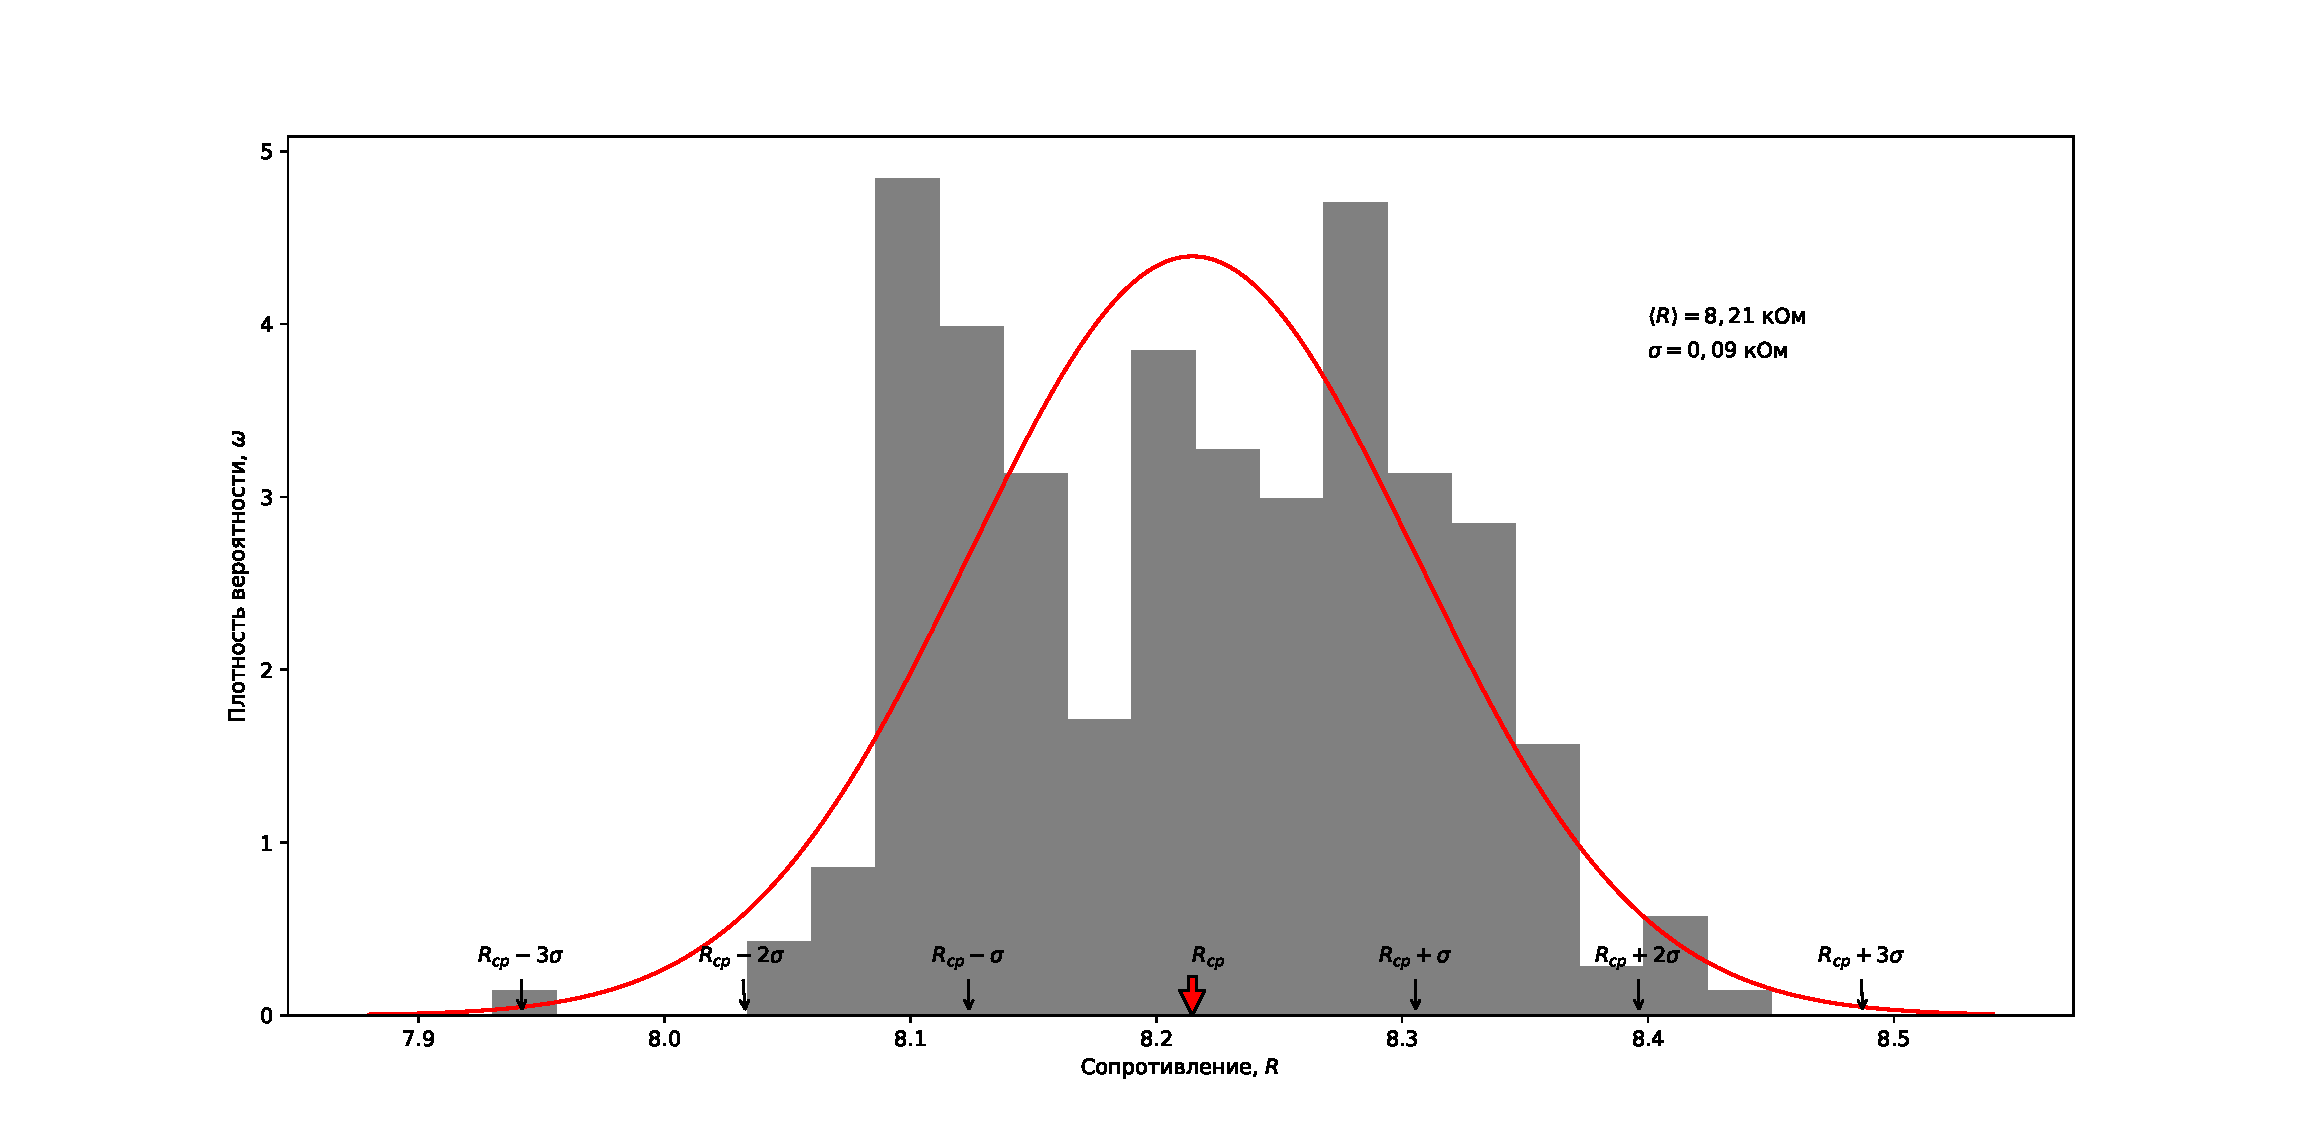
\includegraphics[width=1.1\linewidth]{m=20.pdf}
\caption{Гистограмма для $ m = 20 $}\label{gist20}

\end{figure}

\begin{figure}
	
	
	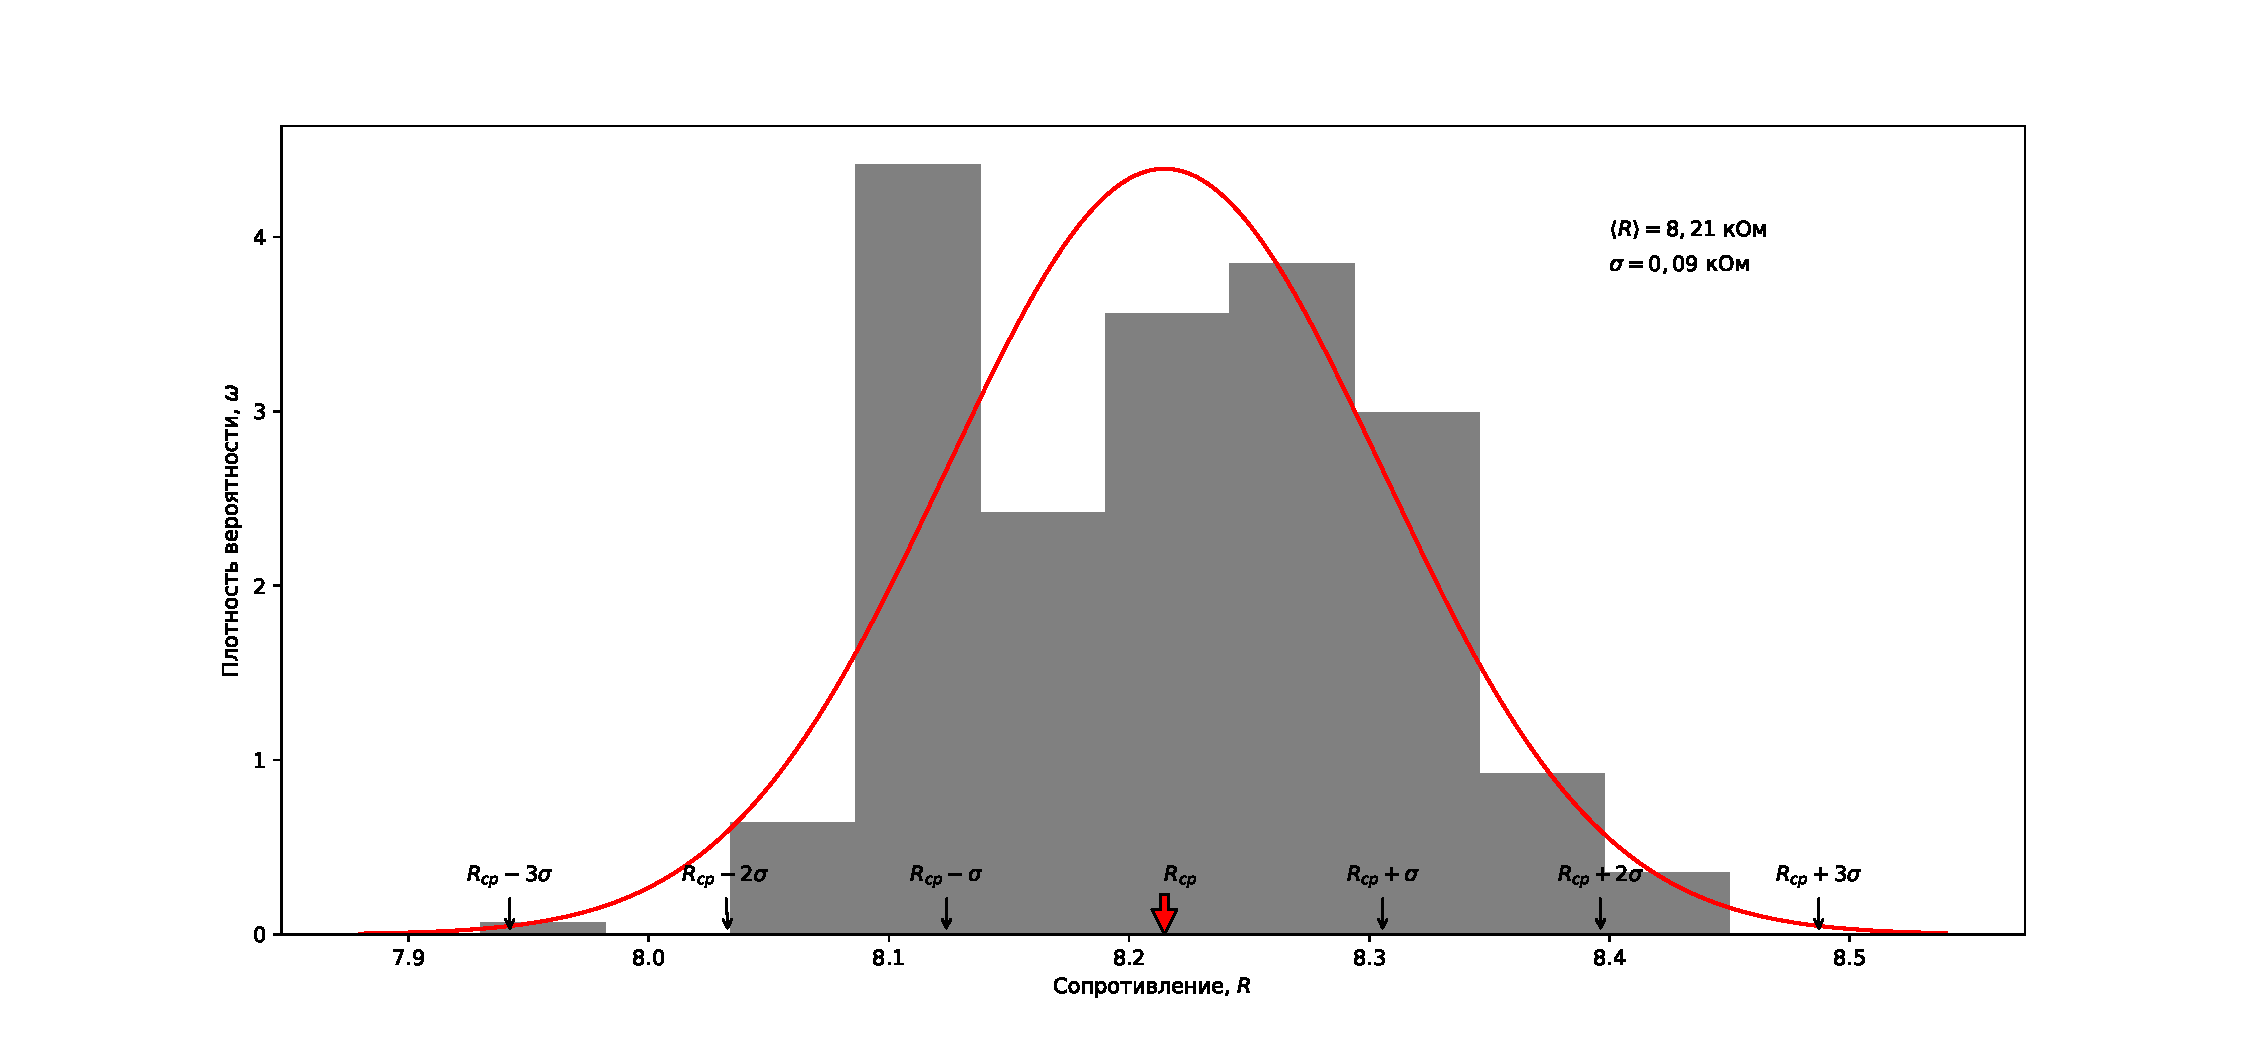
\includegraphics[width=1.08\linewidth]{m=10.pdf}
	\caption{Гистограмма для $ m = 10 $}\label{gist10}
	
\end{figure}
\newpage
Нормальное распределение описывается следующей формулой:

\begin{equation}
y = \frac{1}{\sqrt{2\pi} \sigma} e^{-\frac{\left(R - \langle R \rangle \right)^2}{2\sigma^2}}
\end{equation}

Эта функция также изображена на рис. \ref{gist20} и \ref{gist10}. Видно, что гистограмма практически соответствует этой зависимости. Теоретическая вероятность попадания измерений в интервал от $ \langle R \rangle - \sigma $ до $ \langle R \rangle + \sigma $ равна $ 68\% $, а в интервал от $ \langle R \rangle - 2\sigma $ до $ \langle R \rangle + 2\sigma $ соответственно -- $ 95\% $.

\section{Обсуждение результатов и выводы}

В ходе работы мы получили, что величина сопротивления резистора, наугад выбранного из данного набора, попадает в интервал $ 8,21 \pm 0,09 $ кОм с вероятностью $ 61\% $,  в интервал $ 8,21 \pm 0,18 $ кОм с вероятностью $ 97\% $,  в интервал $ 8,21 \pm 0,27 $ кОм с вероятностью $ 99\% $.\\

\noindent Таким образом, величины всех сопротивлений укладываются в 5-процентный интервал $ \left( \langle R \rangle \pm 3\sigma \right)  $.\\

\noindent Однако, как можно заметить, измеренные результаты неидеально описываются нормальным распределением. Это можно объяснить неточностью метода измерения, в том числе окислением контактов резисторов и/или измерительных приборов. Также незначительный вклад в отклонение вносит изменение сопротивления резисторов в зависимости от температуры окружающей среды.




\end{document}